\subsection{Caso d'uso UC11: Stampa infografica}
\begin{figure}[h] 
	\centering 
	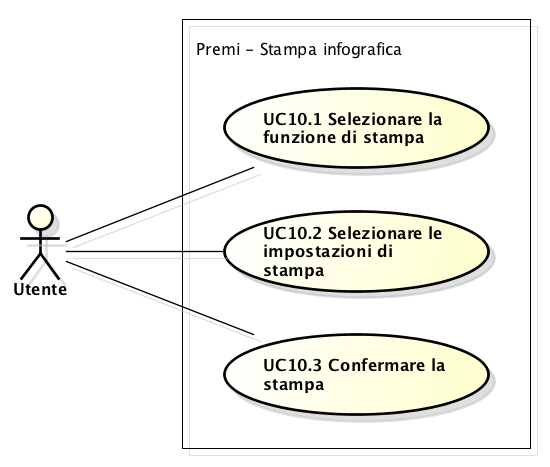
\includegraphics[scale=0.45] {img/UC11.png} 
	\caption{UC11 - Stampa infografica} 
\end{figure}

\begin{itemize}
	\item \textbf{Attori:} Utente;
	\item \textbf{Scopo e descrizione:} L'utente ha creato un'infografica e vuole stamparla;
	\item \textbf{Precondizione:} Il sistema è in attesa che l'utente selezioni la funzione stampa;
	\item \textbf{Flusso degli eventi:}
	\begin{enumerate}
		\item L'utente seleziona la funzione stampa [UC11.1];
		\item L'utente seleziona le impostazioni di stampa [UC11.2];
		\item L'utente conferma la stampa [UC11.3].
	\end{enumerate}
	\item \textbf{Postcondizione:} Il sistema ha mandato in stampa l'infografica.
\end{itemize}

\subsection{Caso d'uso UC11.1: Selezionare la funzione di stampa}
\begin{itemize}
	\item \textbf{Attori:} Utente;
	\item \textbf{Scopo e descrizione:} L'utente seleziona dall'apposito menù la funzione di stampa per stampare l'infografica;
	\item \textbf{Precondizione:} Il sistema è in attesa che l'utente selezioni la funzione stampa;
	\item \textbf{Postcondizione:} Il sistema apre la finestra di dialogo per la stampa.
\end{itemize}

\subsection{Caso d'uso UC11.2: Selezionare le impostazioni di stampa}
\begin{figure}[h] 
	\centering 
	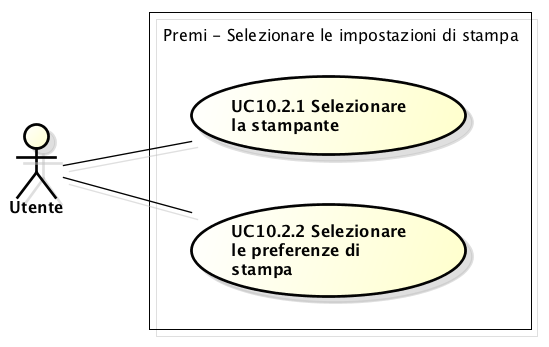
\includegraphics[scale=0.45] {img/UC11.2.png} 
	\caption{UC11.2 - Selezione impostazioni di stampa} 
\end{figure}

\begin{itemize}
	\item \textbf{Attori:} Utente;
	\item \textbf{Scopo e descrizione:} L'utente deve selezionare le impostazioni per la stampa dell'infografica;
	\item \textbf{Precondizione:} Il sistema permette all'utente di selezionare le impostazioni desiderate;
	\item \textbf{Flusso di eventi:}
	\begin{enumerate}
		\item L'utente seleziona quale stampante usare [UC11.2.1]
		\item L'utente seleziona le preferenze di stampa fornite dalla stampante[UC11.2.2]
	\end{enumerate}
	\item \textbf{Postcondizione:} Il sistema registra tutte le impostazioni selezionate dall'utente.
\end{itemize}
	
	\subsection{Caso d'uso UC11.2.1: Selezionare la stampante}
	\begin{itemize}
		\item \textbf{Attori:} Utente;
		\item \textbf{Scopo e descrizione:} L'utente seleziona quale stampante installata nel sistema usare;
		\item \textbf{Precondizione:} Il sistema è in attesa che l'utente selezioni la stampante da usare;
		\item \textbf{Postcondizione:} Il sistema registra la scelta fatta dall'utente.
	\end{itemize}
	
	\subsection{Caso d'uso UC11.2.2: Selezionare le preferenze di stampa}
	\begin{itemize}
		\item \textbf{Attori:} Utente;
		\item \textbf{Scopo e descrizione:} L'utente seleziona le preferenze di stampa fornite dai driver della stampante stessa;
		\item \textbf{Precondizione:} Il sistema è in attesa che l'utente selezioni le preferenze da usare;
		\item \textbf{Postcondizione:} Il sistema registra la scelte fatte dall'utente.
	\end{itemize}

\subsection{Caso d'uso UC11.3: Conferma di stampa}
\begin{itemize}
	\item \textbf{Attori:} Utente;
	\item \textbf{Scopo e descrizione:} L'utente conferma la stampa dell'infografica;
	\item \textbf{Precondizione:} Il sistema ha ricevuto la richiesta di stampa dell'infografica;
	\item \textbf{Postcondizione:} Il sistema ha mandato in stampa l'infografica.
\end{itemize}

\newpage